%%% In this section, you will describe all of the various artifacts that you will generate and maintain during the project life cycle. Describe the purpose of each item below, how the content will be generated, where it will be stored, how often it will be updated, etc. Replace the default text for each section with your own description. Reword this paragraph as appropriate.

\subsection{Major Documentation Deliverables}
The major deliverables are this project charter, system requirements specification, architectural design specification, and detailed design specification. These are the main documents that will be turned in during the first half of the project. Each of these document will be prepared with the co-operation of the whole team and stored in team's github as we move forward with the project. These documents will also be updated as needed during the course of the project. 

\subsubsection{Project Charter}
This document will be maintained as a team and updated during each sprint if any requirement is edited, added or removed. The initial version will be delivered on October 3rd, 2022 and the final version will be delivered along with the complete project on May of 2023.

\subsubsection{System Requirements Specification}
This document will be maintained as a team and updated as needed. The requirements will not be edited as much as other documents, but it will be updated if the team decides to add or remove some parts. The initial version will be delivered towards the end of October 2022 and the final version will be delivered along with the complete project on May of 2023.

\subsubsection{Architectural Design Specification}
This document will be maintained as a team and updated frequently during the first half of the project. In the second half as we progress in the project and we have a solid structure for the project, it will be updated few times. The initial version will be delivered on November of 2022 and the final version will be delivered along with the complete project on May of 2023.

\subsubsection{Detailed Design Specification}
This document will be maintained as a team and updated frequently during the initial stages. However, it will not be updated much after the completion of the design of the project. If a major change happens in the project, it will be updated accordingly. The initial version will be delivered on October 3rd, 2022 and the final version will be delivered along with the complete project on May of 2023.

\subsection{Recurring Sprint Items}
\subsubsection{Product Backlog}
The items will be added after the discussion with the whole team after splitting up tasks so that no item on the backlog is too big. These items will be prioritized according to the need for the software. The decisions will be based on the majority vote. The software to maintain and share the product backlog with team members and stakeholders will be Jira.

\subsubsection{Sprint Planning}
Each sprint will be planned before the beginning of the sprint. The backlog can be updated during the sprint. In Senior Design 1, there will be 4 sprints. In Senior Design 2, there will also be 4 sprints.

\subsubsection{Sprint Goal}
The Sprint goal is decided by the group together with some feedback from the sponsor and customers of the project. 

\subsubsection{Sprint Backlog}
The team together will decide the backlog items and they will be kept in the Jira Board by the scrum master. The backlog will be maintained by the whole team as they progress in their allocated tasks with options like in-progress, done, etc.

\subsubsection{Task Breakdown}
Individual task will be assigned by group discussion and the preference of each member. If there is a conflict, then the group leader for the sprint will decide how the conflicted task will be divided. Time spent on tasks will be documented using man hour.

\subsubsection{Sprint Burn Down Charts}
The scrum master will be responsible for generating the burn down charts for each sprint. The Jira Board has a feature to keep track of time spent on each task and Jira Board will create a burn down chart accordingly.

\begin{figure}[h!]
    \centering
    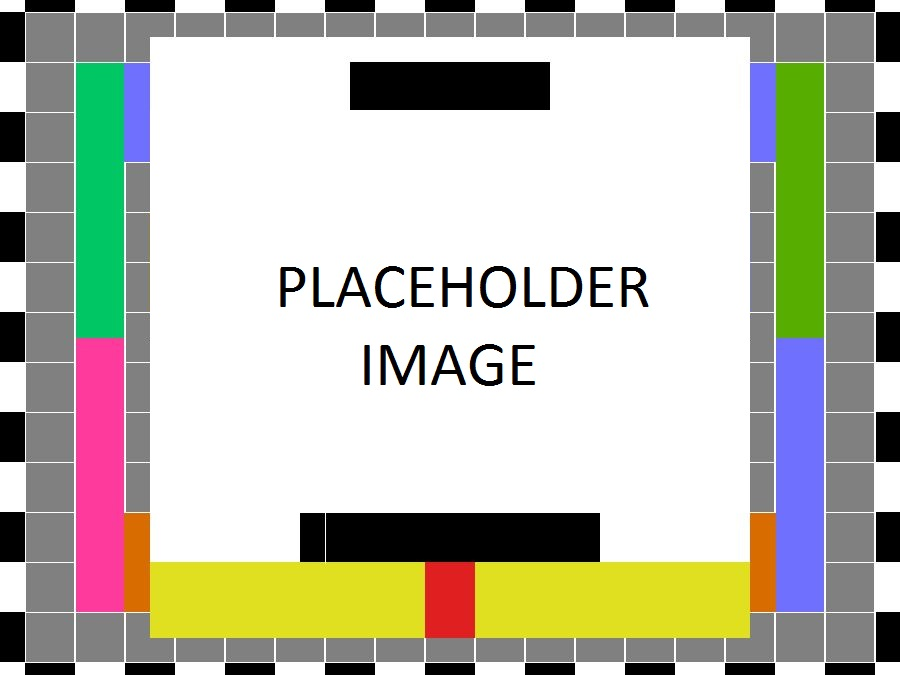
\includegraphics[width=0.5\textwidth]{images/test_image}
    \caption{Example sprint burn down chart}
\end{figure}

\subsubsection{Sprint Retrospective}
How will the sprint retrospective be handled as a team? When will this discussion happen after each sprint? What will be documented as a group and as individuals, and when will it be due?
The Sprint retrospective will be handled after the day of completion of each sprint. As a group, problems faced, lessons learned, ways to improve communication and the allocation of task will be documented. As individuals, lessons learned and peer reviews will be documented. These are due according to the schedule provided by the professor.

\subsubsection{Individual Status Reports}
In the progress discussion meeting, each member will discuss the progress made by them and the problems they faced. The key items that will be included in the report will be which items they have worked on, problems they faced, if they need any assistance, etc.

\subsubsection{Engineering Notebooks}
The engineering notebook will be updated after a change is brought up in the project. At a minimum, it will be updated bi-weekly which is the length of each sprint. There will be no minimum amount of pages. Team members will be each others' witness and will keep each other accountable.

\subsection{Closeout Materials}
\subsubsection{System Prototype}
The system prototype will include Acoustic and RF detecting sensor station utilizing a raspberry pi connected to a microcontroller and ADC chain. This chain will connect to an RF detection circuit as well as a four array acoustic sensor tower. Currently, we have decided not to have Prototype Acceptance Test. The protype will be demonstrated off-site. We have shortlisted several locations at UTA and will be decided later on for the demonstration. Currently, we have not decided on whether we will have a Field Acceptance Test or not.

\subsubsection{Project Poster}
Currently, this has not been discussed and will be done in the later part of the project.

\subsubsection{Web Page}
The project web page will include the GUI of real time drone tracking. The tracking will be shown suing satellite image/Google Maps and location services will be displayed of the trackers. The completion of the web page also highlights the completion of the project and it will be delivered at closeout as a complete project.

\subsubsection{Demo Video}
Demo video will show the real time drone tracking mechanism. The website will also be shown. We will not include a B-reel footage. The demo video will be around 10 minutes long and it will cover the mechanism used by the drone tracker , sensors used to detect drones and real time drone tracking and working of our website.

\subsubsection{Source Code}
Source code will be maintained through github which is a version control system. Source code will be accessible to the sponsor directly through github. Currently, there is no plan for the project to be open sourced.

\subsubsection{Source Code Documentation}
The source code will be well commented and proper formatting will be used by every coder. We will be using Doxygen and we will provide the documentation in pdf format.

\subsubsection{Hardware Schematics}
Currenlty, we are not sure whether we will use the PCBs or not. We will update this section as we progress forward in the project. 

\subsubsection{Installation Scripts}
The web application of the project will be present online and will be accessible easily to the customer. Once the sensors are activated, data generation will begin and stored in the database. The data matching the criteria for drones will be then displayed on the web page which can be easily viewed by the customer. The customer will need to place multiple sensor towers in the desired location for the data generation to begin. User guide will be provided along with the completion of the project for the use of the product.  

\subsubsection{User Manual}
A digital user manual will be created towards the end of the project that describes all major parts of the project. A short demo video will also be provided on how to use the product.
